\subsubsection{Toric code}
Similarly, a hypergraph product code of two ring codes can be 
generated. We call this code the "Toric code".\\
\begin{figure}[h!]
	\begin{center}
	\captionsetup{justification=centering,margin=2cm}
	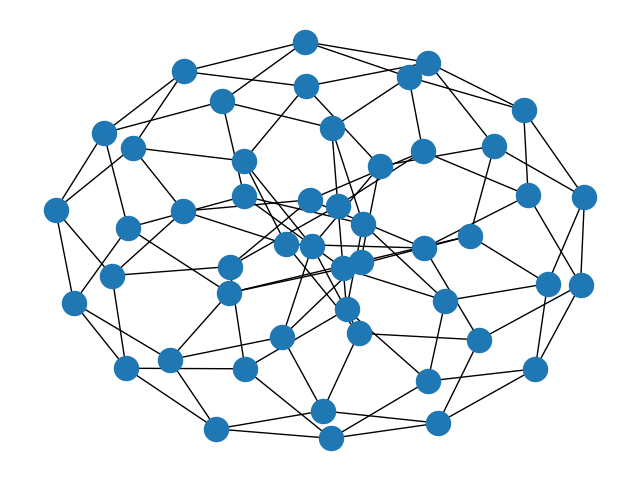
\includegraphics[scale=0.4]{./img/figures/toric_5_graph.png}\\
	\caption{Graph for [[49,1,7]] toric code}
        
	\label{fig: toric_graph}
	\end{center}
\end{figure}
Notably, this resembles a donut, or torus.
The logical operators on the toric code are loops, so a circle of 
'errors' on nodes is a logical X operator, and a circle of 'errors'
on faces is a logical Z operator.
\newpage